% Visual system of the Team AGX deck: the poster's identity (FIVE SENSORS. ONE DECISION.), the report's semantic palette,
% Lato loaded from the same TTF files matplotlib uses, warm paper background, navy full-bleed frames for emphasis.
% Compile with lualatex. Components: \takeaway \heronum \metriccard \callout \resultbadge \verificationcell/\vrow \processstream \sensorvisual \talk
\usepackage{iftex}
\ifluatex
  % Lato from the same TTF files matplotlib uses, so figure text and slide text are one typeface
  \usepackage{fontspec}
  \setsansfont[Path=/usr/share/fonts/truetype/lato/, Extension=.ttf, UprightFont=Lato-Regular, BoldFont=Lato-Bold, ItalicFont=Lato-Italic, BoldItalicFont=Lato-BoldItalic]{Lato}
  \newfontfamily\latoblack[Path=/usr/share/fonts/truetype/lato/, Extension=.ttf, UprightFont=Lato-Black, BoldFont=Lato-Black]{Lato}
  \setmonofont[Path=/usr/share/fonts/truetype/liberation/, Extension=.ttf, UprightFont=LiberationMono-Regular, BoldFont=LiberationMono-Bold, Scale=0.9]{LiberationMono}
\else
  % pdflatex fallback (texlive-luatex not installed): Helvetica-metric sans; \latoblack becomes bold
  \usepackage[T1]{fontenc}\usepackage[scaled=0.96]{helvet}\renewcommand{\familydefault}{\sfdefault}
  \newcommand{\latoblack}{\sffamily\bfseries}
\fi
\usepackage{tikz,xcolor,colortbl,booktabs,array,graphicx,amsmath}
\usetikzlibrary{calc,positioning,arrows.meta,shapes.misc}
\graphicspath{{figures/}{../report/figures/}}

% ---------------------------------------------------------------- semantic palette (figstyle.py)
\definecolor{ink}{HTML}{1B2A41}        % fusion / context / dark slides
\definecolor{blue}{HTML}{2E5C9E}       % IR + depth, body
\definecolor{bluelight}{HTML}{6F97D1}  % hands
\definecolor{orange}{HTML}{D9772B}     % thermal
\definecolor{teal}{HTML}{1F7F7A}       % skeleton
\definecolor{seagreen}{HTML}{5FB3A9}   % IMU
\definecolor{violet}{HTML}{6B4FA0}     % radar / recording order
\definecolor{red}{HTML}{B4433A}        % negative result
\definecolor{gray}{HTML}{8A929B}       % baseline (fills)
\definecolor{graytext}{HTML}{4B535E}   % secondary text
\definecolor{graylight}{HTML}{D6DBE1}
\definecolor{band}{HTML}{F3F1EC}
\definecolor{paper}{HTML}{FBFAF7}
\definecolor{green}{HTML}{3D8B5A}

% ---------------------------------------------------------------- beamer skeleton
\usetheme{default}
\setbeamertemplate{navigation symbols}{}
\setbeamercolor{background canvas}{bg=paper}
\setbeamercolor{normal text}{fg=ink}
\setbeamercolor{structure}{fg=ink}
\setbeamercolor{item}{fg=blue}
\setbeamerfont{normal text}{size=\normalsize}
\setbeamersize{text margin left=0.6cm, text margin right=0.6cm}
\setbeamertemplate{frametitle}{\vspace{0.3cm}{\latoblack\fontsize{14.5}{16}\selectfont\color{ink}\insertframetitle\par}\vspace{0.05cm}}
\setbeamertemplate{footline}{\hspace{0.6cm}{\fontsize{6}{7}\selectfont\color{graytext}FIVE SENSORS. ONE DECISION.\quad Team AGX, CUHK-X Challenge 2026}\hfill{\fontsize{6}{7}\selectfont\color{graytext}\insertframenumber}\hspace{0.6cm}\vspace{0.18cm}}
\setbeamertemplate{itemize item}{\textcolor{blue}{\rule[0.1em]{0.35em}{0.35em}}}
\setbeamertemplate{note page}{\vspace{0.4cm}{\fontsize{9}{11}\selectfont\insertnote}}

% ---------------------------------------------------------------- components
% \takeaway{sentence}: the one sentence under the title (the only text a viewer needs)
\newcommand{\takeaway}[1]{{\fontsize{9}{11}\selectfont\color{graytext}#1\par}\vspace{0.12cm}}
% \heronum[size]{big}{label}: a very large number with a small label under it
\newcommand{\heronum}[3][26]{\begin{minipage}[t]{\linewidth}\raggedright{\latoblack\fontsize{#1}{#1}\selectfont\color{ink}#2\par}\vspace{0.06cm}{\fontsize{7.5}{9}\selectfont\color{graytext}\bfseries #3\par}\end{minipage}}
% \heronumc[size]{big}{label}: centred variant
\newcommand{\heronumc}[3][26]{\begin{minipage}[t]{\linewidth}\centering{\latoblack\fontsize{#1}{#1}\selectfont\color{ink}#2\par}\vspace{0.06cm}{\fontsize{7.5}{9}\selectfont\color{graytext}\bfseries #3\par}\end{minipage}}
% \metriccard{big}{label}: a number on a band card
\newcommand{\metriccard}[2]{\begin{tikzpicture}\node[fill=band, rounded corners=2pt, inner sep=5pt, text width=2.6cm, align=center]{{\latoblack\fontsize{18}{18}\selectfont\color{ink}#1}\\[1pt]{\fontsize{7.5}{9}\selectfont\color{graytext}\bfseries #2}};\end{tikzpicture}}
% \callout{text}: a band box with a navy rule on the left
\newcommand{\callout}[1]{\begin{tikzpicture}\node[fill=band, inner sep=5pt, text width=\linewidth-10pt, align=left]{\fontsize{8.5}{10.5}\selectfont #1};\draw[ink, line width=2pt] (current bounding box.north west) -- (current bounding box.south west);\end{tikzpicture}}
% \resultbadge{text}: navy pill with white text
\newcommand{\resultbadge}[1]{\tikz[baseline=(b.base)]\node[fill=ink, text=white, rounded corners=6pt, inner xsep=6pt, inner ysep=3pt, font=\fontsize{8}{9}\selectfont\bfseries] (b) {#1};}
% \okbadge{text}: green-edged pill
\newcommand{\okbadge}[1]{\tikz[baseline=(b.base)]\node[draw=green, line width=0.8pt, text=green, rounded corners=6pt, inner xsep=6pt, inner ysep=3pt, font=\fontsize{8}{9}\selectfont\bfseries] (b) {#1};}
% verification matrix cells (gen/verification.tex emits \vrow lines)
\newcommand{\verificationcell}[2]{\cellcolor{#1}{\color{ink}\bfseries #2}}
\newcommand{\vrow}[5]{\textbf{#1} & {\color{graytext}#2} & #3 & \verificationcell{band}{#4} & \verificationcell{band}{\color{green}#5}\\}
% \processstream: five specialists -> fusion -> context -> one decision, as a TikZ line (text slides)
\newcommand{\processstream}{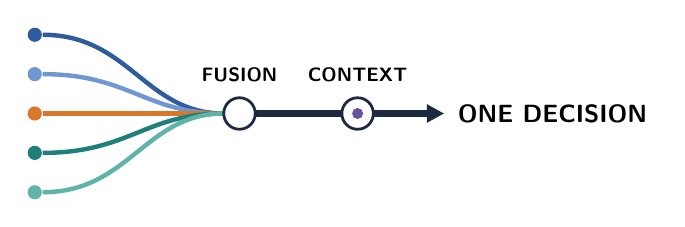
\begin{tikzpicture}[x=1cm, y=1cm]
  \foreach \c/\i in {blue/0, bluelight/1, orange/2, teal/3, seagreen/4}{\fill[\c] (0, 1.0-0.5*\i) circle (0.09); \draw[\c, line width=1.6pt] (0.1, 1.0-0.5*\i) .. controls (1.2, 1.0-0.5*\i) and (1.4, 0) .. (2.4, 0);}
  \draw[ink, fill=white, line width=1pt] (2.6, 0) circle (0.2); \node[anchor=south, font=\fontsize{7.5}{8}\selectfont\bfseries] at (2.6, 0.28) {FUSION};
  \draw[ink, line width=2.2pt] (2.8, 0) -- (3.9, 0); \draw[ink, fill=white, line width=1pt] (4.1, 0) circle (0.2); \fill[violet] (4.1, 0) circle (0.07); \node[anchor=south, font=\fontsize{7.5}{8}\selectfont\bfseries] at (4.1, 0.28) {CONTEXT};
  \draw[ink, line width=2.2pt, -{Triangle[length=2.2mm, width=2.2mm]}] (4.3, 0) -- (5.2, 0); \node[anchor=west, font=\latoblack\fontsize{9}{9}\selectfont] at (5.25, 0) {ONE DECISION};
\end{tikzpicture}}
% \sensorvisual[width]{file}: a generated figure
\newcommand{\sensorvisual}[2][\textwidth]{\includegraphics[width=#1]{#2}}
% \talk{script}{one sentence}{likely challenge}{answer}: speaker notes
\newcommand{\talk}[4]{\note{\textbf{Script.} #1\par\medskip\textbf{One sentence.} #2\par\medskip\textbf{Likely challenge.} #3\par\medskip\textbf{Answer.} #4}}
% \navytitle{...}: display type on the navy slides
\newcommand{\navytitle}[1]{{\latoblack\fontsize{26}{28}\selectfont\color{white}#1\par}}
